\documentclass[12pt]{article}
\usepackage[a4paper, total={6in, 9in}]{geometry}
\usepackage{graphicx}
\graphicspath{ {./images/output/} }
\usepackage{caption}
\usepackage[english]{babel}
\usepackage{titling}
\usepackage{float}
\usepackage{amsmath}
\usepackage{minted}
\usepackage{multicol}
% \usepackage{array}
% \usepackage{setspace}
% \usepackage{placeins}
\usepackage{parskip}

% \usepackage{lipsum}

\title{Study and Simulation of 1-Bit SRAM Using Microwind}
\author{}
\date{}

\pagenumbering{gobble}
\begin{document}
\vspace*{\fill}
\begin{center}

    \emph{Heaven's Light is Our Guide} \\
    \textbf{Rajshahi University of Engineering and Technology} \\

    \begin{figure}[H]
        \centering
        
\includegraphics[scale=.34]{images/RUET_logo.png}
        \label{fig:ruet_logo}
    \end{figure}
    \vspace{5mm}

    \textbf{Course Code}\\
    ECE 4128\\
    \vspace{3mm}
    \textbf{Course Title}\\
    VLSI Design

    \vspace{5mm}
    \textbf{Experiment Date:} {July 4, 2025},\\
    \textbf{Submission Date:} {August 11, 2025}\\

    \vspace{5mm}
    \textbf{Lab Report 2: \\
        Implementation of NMOS Ratio-less Inverter.}

    \vspace{15mm}

    \begin{tabular}{c|c}
        \textbf{Submitted to} & \textbf{Submitted by} \\
        Moloy Kumar Ghosh     &                       \\
        Lecturer              &                       \\
        Dept of ECE, RUET     & Md. Tajim An Noor     \\
        \&                    & Roll: 2010025         \\
        Md. Faysal Ahamed     &                       \\
        Lecturer              &                       \\
        Dept of ECE, RUET     &                       \\
    \end{tabular}

\end{center}
\vspace*{\fill}


\pagebreak

\tableofcontents

\pagebreak
\pagenumbering{arabic}
\maketitle

\section*{Theory}
\addcontentsline{toc}{section}{Theory}
A 1‑bit SRAM cell is most often realised with a 6‑transistor (6T) topology: two cross‑coupled CMOS inverters create a bistable latch that holds complementary storage nodes \(Q\) and \(\overline{Q}\). Two NMOS access transistors, enabled by the word line \(WL\), connect the latch to the differential bit‑lines \(BL\) and \(\overline{BL}\) \cite{WesteHarris, Rabaey}.

\begin{itemize}
  \item Hold: With \(WL=0\) the access transistors are off and the latch preserves its state by positive feedback.
  \item Write: With \(WL=1\) forcing \(BL/\overline{BL}=0/1\) drives the cell to store a logical ‘0’ at \(Q\); conversely forcing \(BL/\overline{BL}=1/0\) writes a ‘1’.
  \item Read: Both bit‑lines are precharged high. Asserting \(WL=1\) weakly discharges the bit‑line tied to the internal ‘0’ node, producing a small differential \(\Delta V\) that a sense amplifier detects; ideally the stored state is not destroyed (practical read behaviour depends on sizing and device nonidealities) \cite{CalhounChandrakasan}.
\end{itemize}

Authenticity check: the above description and operation modes are consistent with standard textbook treatments of SRAM fundamentals. Note that the behavioural update equations below are an idealised logical abstraction and do not capture analog effects (finite drive, threshold, body effect, leakage, or read‑disturb) which must be evaluated by transistor‑level simulation \cite{WesteHarris, Rabaey}.

Idealised behavioural update equations (logical model):
\[
  Q(t+1) \;=\; \big(WL\;\cdot\;BL\big) \;+\; \big(\overline{WL}\;\cdot\;Q(t)\big),
\]
\[
  \overline{Q}(t+1) \;=\; \big(WL\;\cdot\;\overline{BL}\big) \;+\; \big(\overline{WL}\;\cdot\;\overline{Q}(t)\big),
\]
where \(\cdot\) denotes logical AND and \(+\) denotes logical OR. During a read (both bit‑lines precharged) the hold term typically dominates.

\begin{figure}[H]
  \centering
  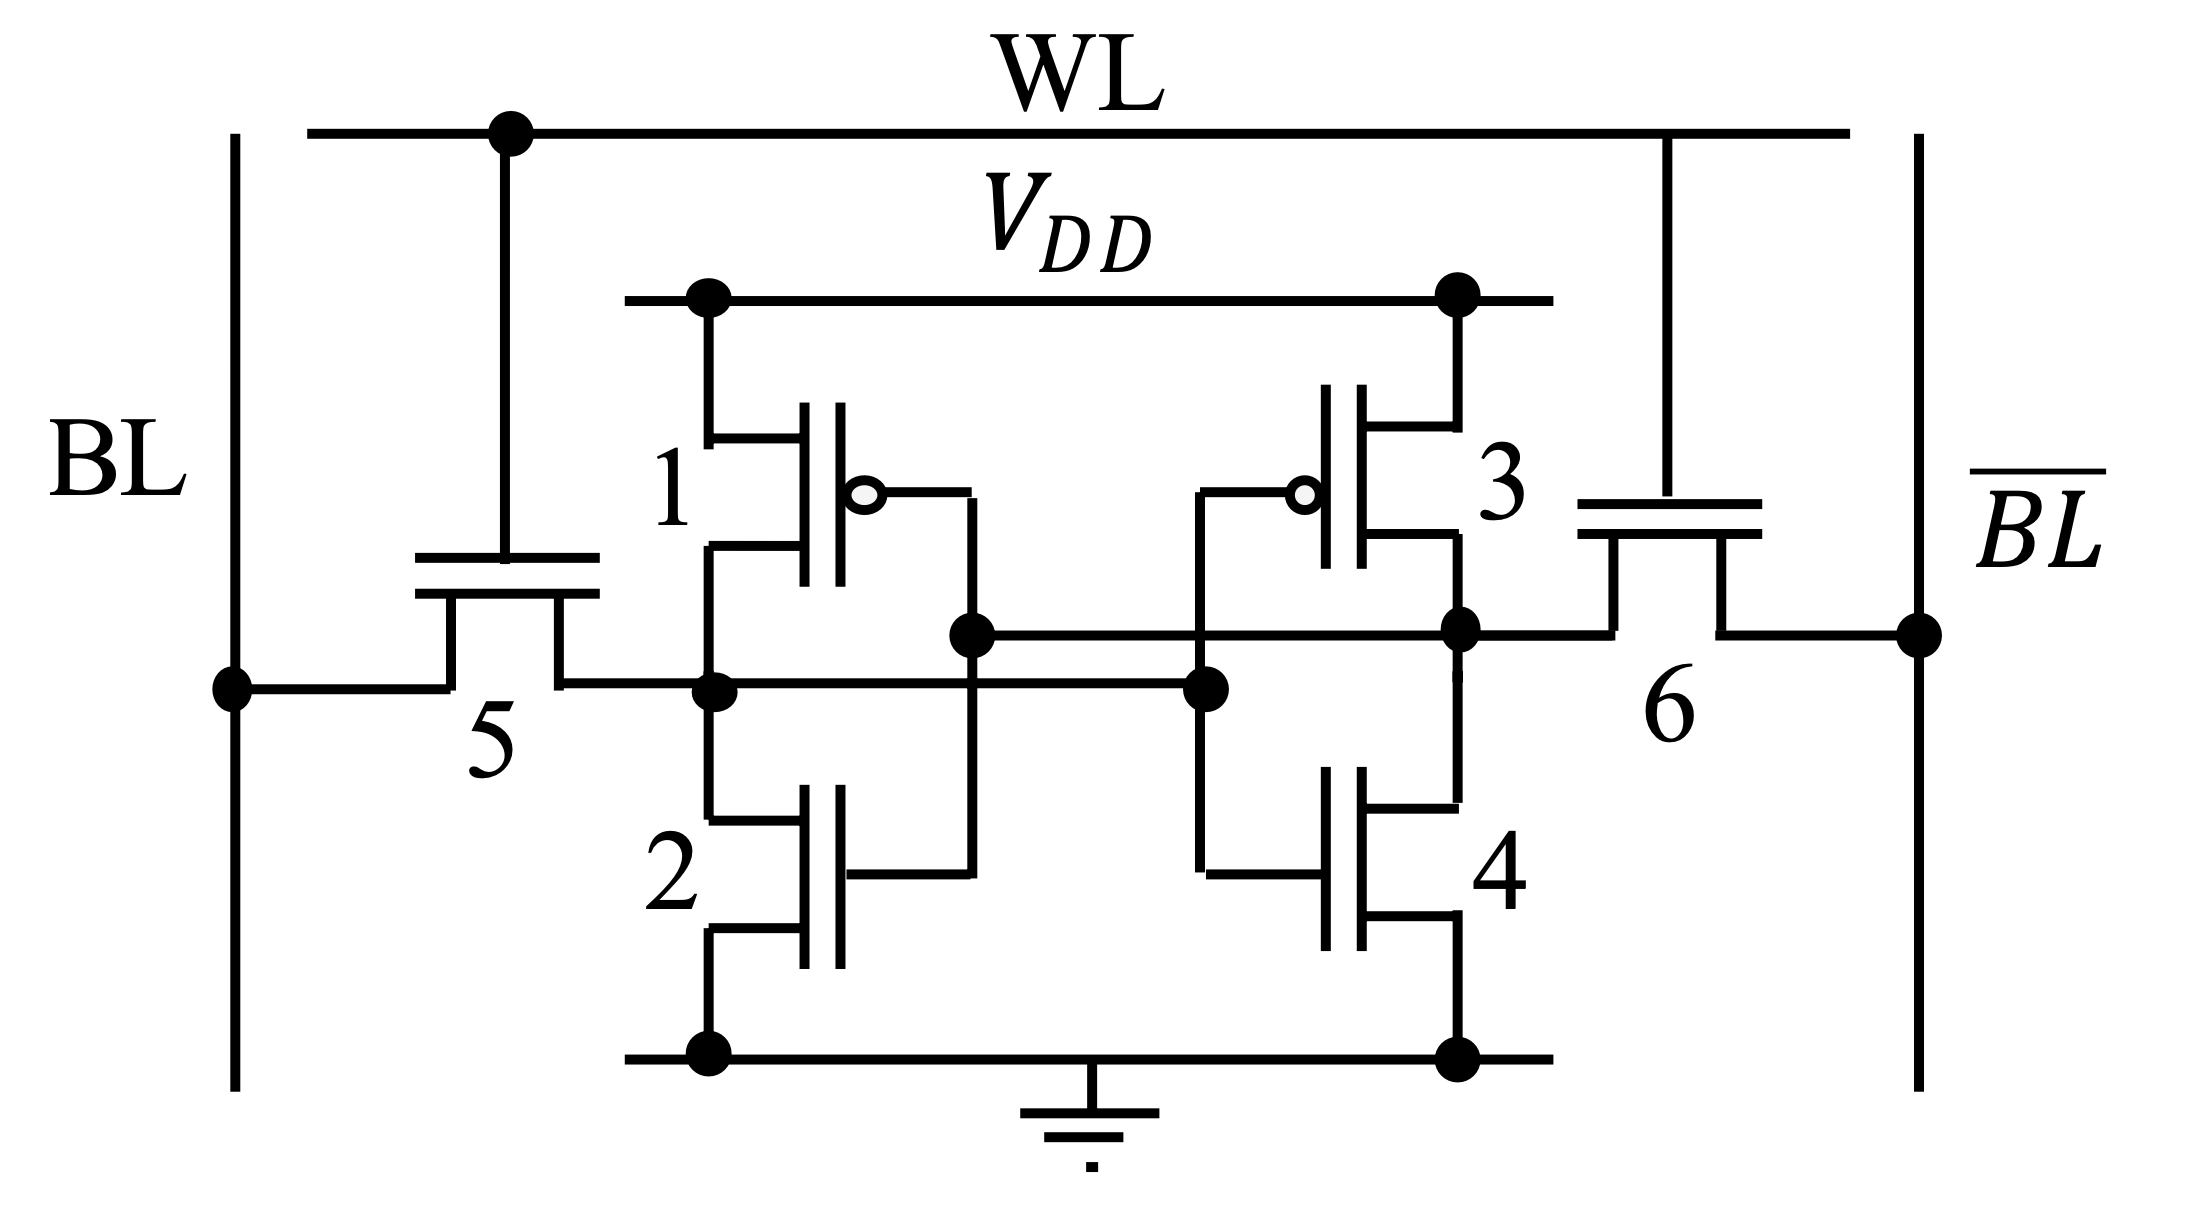
\includegraphics[width=\textwidth]{c.png}
  \caption{Circuit diagram of 1 Bit SRAM cell}
\end{figure}

\begin{table}[H]
  \centering
  \begin{tabular}{|c|c|c|c|c|c|}
    \hline
    WL & BL & $\overline{\text{BL}}$ & Before (Q) & Action                             & After (Q)                    \\
    \hline
    0  & X  & X                      & 0 or 1     & Hold (cell isolated)               & Unchanged                    \\
    \hline
    1  & 1  & 0                      & 0 or 1     & Write '1' (drive nodes)            & 1                            \\
    \hline
    1  & 0  & 1                      & 0 or 1     & Write '0' (drive nodes)            & 0                            \\
    \hline
    1  & 1  & 1*                     & 0 or 1     & Read (bitlines precharged)         & Unchanged (sense $\Delta V$) \\
    \hline
    1  & 0  & 0                      & 0 or 1     & Invalid / weak read (both BLs low) & No reliable change           \\
    \hline
  \end{tabular}
  \begin{flushleft}
    \footnotesize\textit{* precharged.}
  \end{flushleft}
  \caption{SRAM 6T cell operation summary}
  \vspace{2pt}
\end{table}

\section*{Used Tools}
\addcontentsline{toc}{section}{Used Tools}
\begin{itemize}
  \item Microwind
  \item MS Word
  \item MS PowerPoint
  \item \LaTeX
\end{itemize}

\section*{Circuit Schematic in Microwind}
\addcontentsline{toc}{section}{Circuit Schematic in Microwind}

\begin{figure}[H]
  \centering
  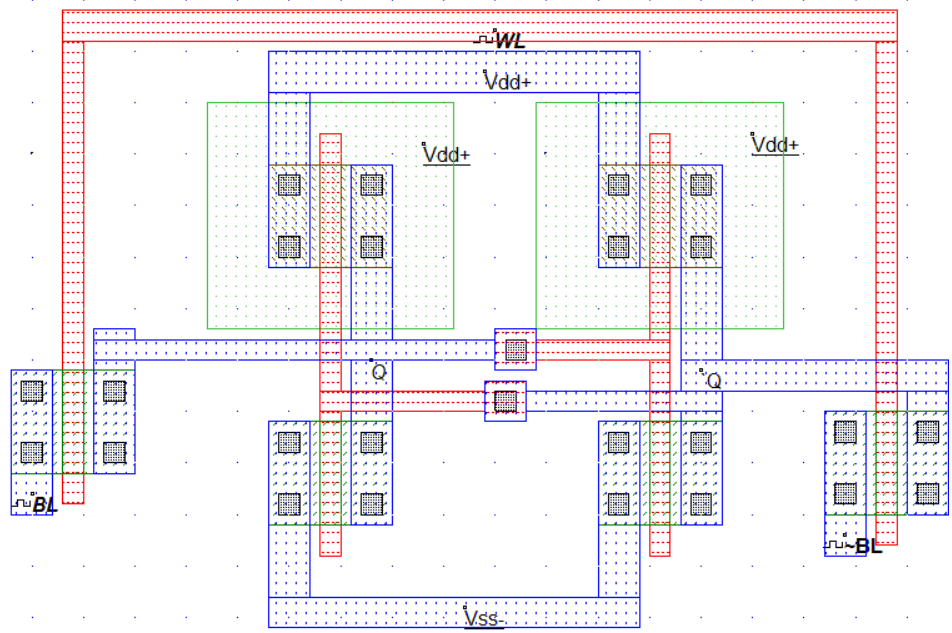
\includegraphics[width=.9\textwidth]{ckt.png}
  \caption{Connection Diagram of 1 Bit SRAM cell in Microwind}
\end{figure}

\section*{Output}
\addcontentsline{toc}{section}{Output}

\begin{figure}[H]
  \centering
  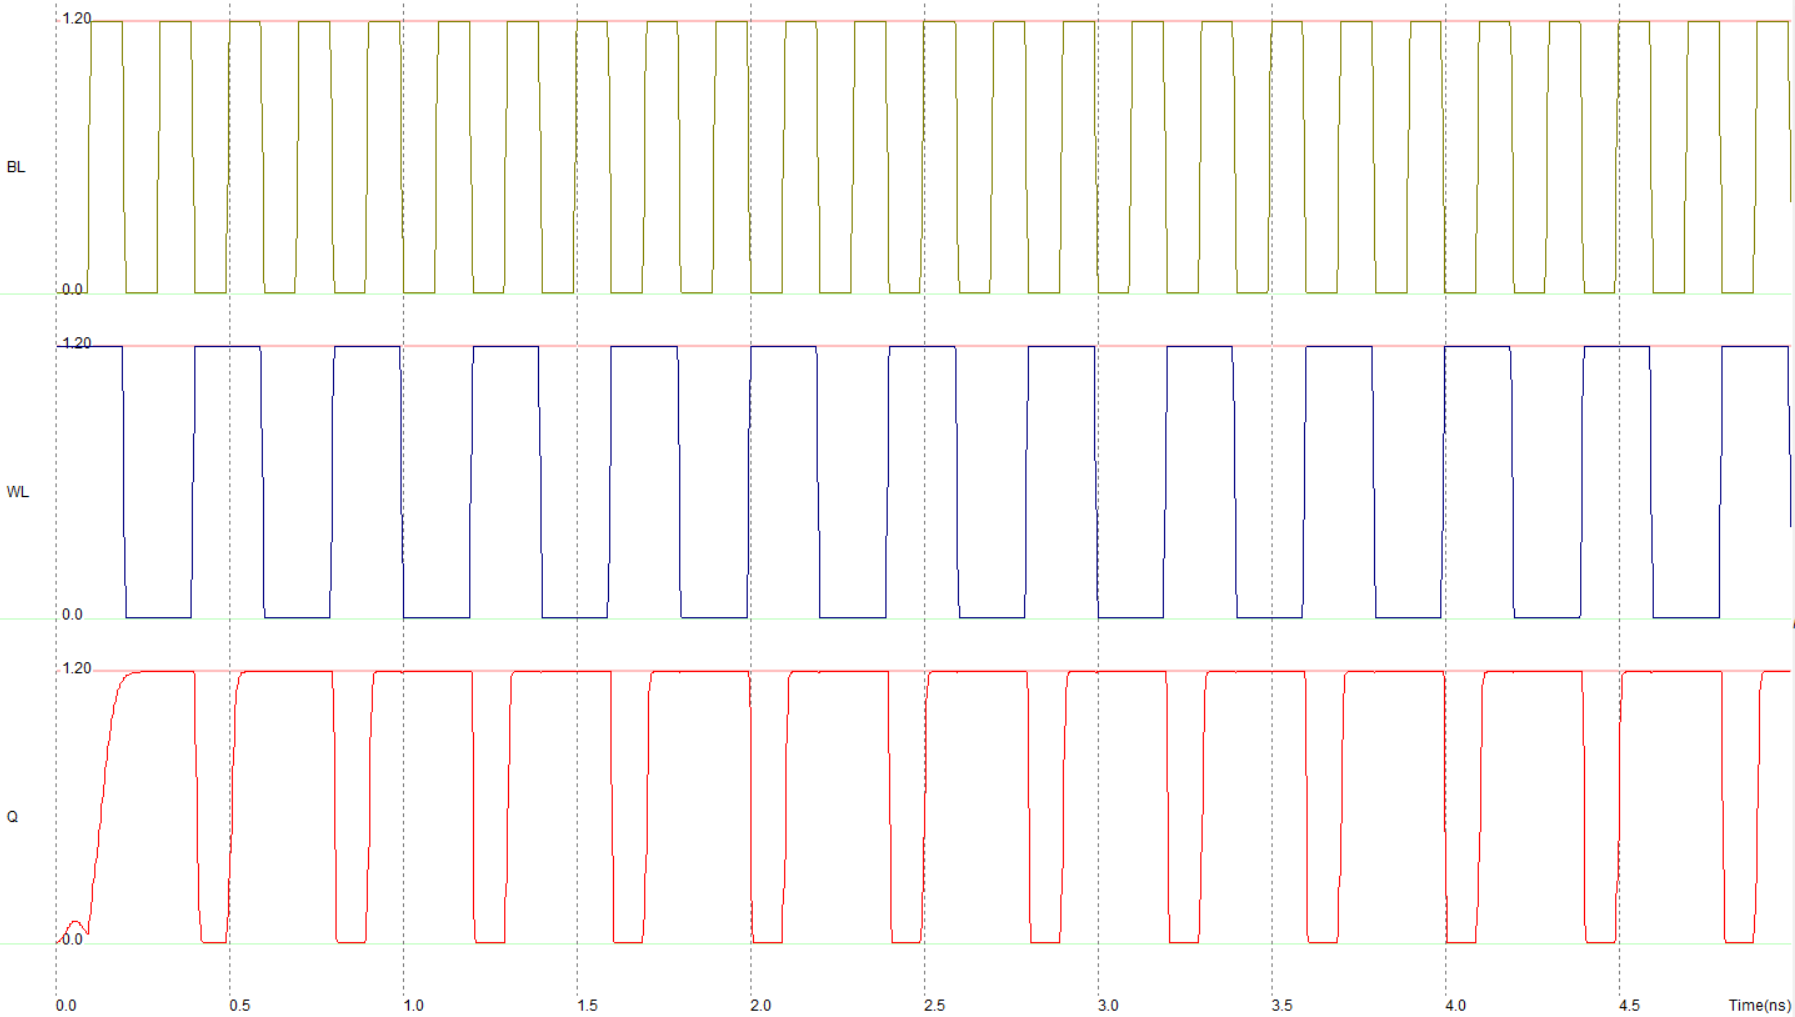
\includegraphics[width=.9\textwidth]{output1.png}
  \caption{Output of the designed 1 Bit SRAM cell in Microwind}
\end{figure}

\subsection*{Output Analysis}
\addcontentsline{toc}{subsection}{Output Analysis}
The Microwind transient simulation confirms correct 1‑bit SRAM operation:

\begin{itemize}
  \item With \(WL=0\) the cell holds its previous state (Q remains constant).
  \item With \(WL=1\) and \(BL/\overline{BL}=1/0\), \(Q\) is written to ‘1’; with \(BL/\overline{BL}=0/1\), \(Q\) is written to ‘0’.
  \item During a read with precharged bit‑lines, asserting \(WL\) produces a small differential on the bit‑lines consistent with the stored value and does not corrupt the cell.
\end{itemize}

Key observations:
\begin{itemize}
  \item Write‑0 is faster than write‑1 due to asymmetric drive strengths.
  \item \(Q\) may not reach \(V_{DD}\) within the WL pulse window, which can limit write‑1 and read margins.
  \item Reads produce only a small BL differential, requiring sensitive sensing and careful transistor sizing.
\end{itemize}

\section*{Discussion}
\addcontentsline{toc}{section}{Discussion}
The results show that cell retention is provided by the positive feedback loop of the cross‑coupled inverters, while the word‑line gated access transistors permit external forcing during write operations and only lightly load the cell during reads. Correct sizing of devices is critical: access transistors must be large enough to reliably overwrite the latch during a write but small enough to avoid compromising the stored value during a read (preserving static noise margin). A symmetric layout and matched inverter device dimensions help equalize bit‑line loading and improve read margin. The transient waveforms follow the expected timing — Q is driven by BL while WL is asserted and remains stable once WL is released — confirming the 6T cell’s functional behaviour.

\section*{Conclusion}
\addcontentsline{toc}{section}{Conclusion}
A 1‑bit, 6‑transistor SRAM cell was implemented and simulated in Microwind. Read, write and hold operations were verified both conceptually and by transient waveform inspection, demonstrating correct operation. The study underlines important design choices for robust SRAM: appropriate transistor sizing, proper bit‑line precharge and equalization, and use of differential sensing to maximize read reliability and scalability.


\bibliographystyle{IEEEtran}
\renewcommand{\bibname}{References}
\addcontentsline{toc}{section}{References}
\bibliography{ref}

\end{document}
